\ylDisplay{Noole kujutis} % Ülesande nimi
{Oleg Košik} % Autor
{piirkonnavoor} % Voor
{2020} % Aasta
{P 8} % Ülesande nr.
{3} % Raskustase
{
% Teema: Valgusõpetus
\ifStatement
Konstrueerige noole $AB$ kujutis kumerläätses. Kas kujutis on tegelik või näiv?
\begin{center}
	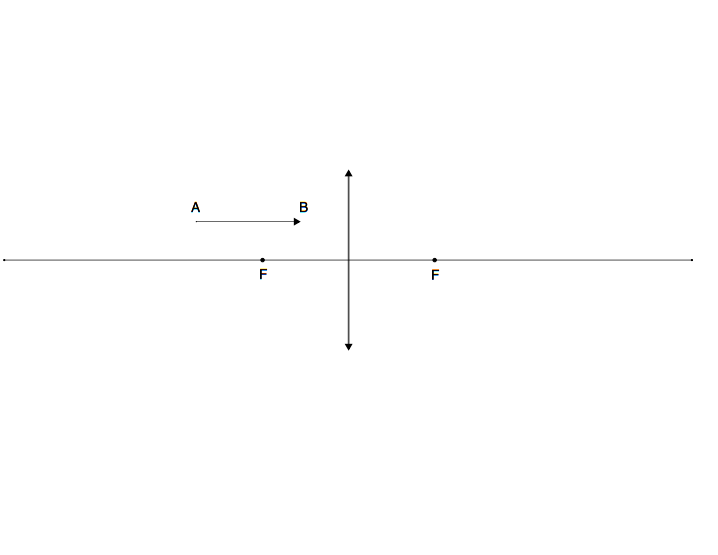
\includegraphics[width=0.5\linewidth]{2020-v2p-08-yl.PNG}
\end{center}
\fi
\ifHint
Ülesande puhul tuleb tähele panna, et osa noolest asub kaugemal kui fookuskaugus ning osa läätsele lähemal, seega on ka tekkiv kujutis osaliselt näiv ning osaliselt tõeline.
\fi
\ifSolution
Konstrueerime kõigepealt punktide $A$ ja $B$ kujutised $A'$ ja $B'$. Noole kujutis asub sirgel $A'B'$, kuid koosneb kahest osast: punktist $A'$ paremale lõpmatusse ning punktist $B'$ vasakule lõpmatusse. Seejuures kujutise parempoolne osa on tegelik ning vasakpoolne näiv.
\begin{center}
	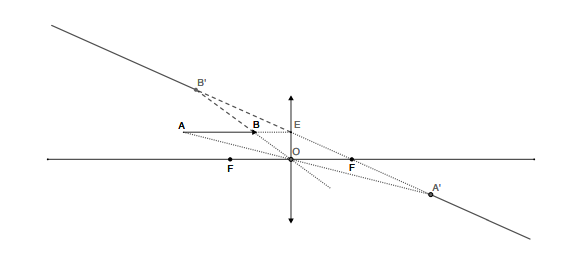
\includegraphics[width=0.5\linewidth]{2020-v2p-08-lah.PNG}
\end{center}
\fi
}
